\documentclass[tikz]{article}
\usepackage{pgfplots}
\pgfplotsset{compat=1.15}
\usepackage{mathrsfs}
\usetikzlibrary{arrows,calc}
\usepackage{tkz-euclide}
\usepackage{tcolorbox}
\usepackage{float}

\pagestyle{empty}

\definecolor{AngleClr}{rgb}{0,0.39215686274509803,0}
\definecolor{ShapeClr}{rgb}{0.6,0.2,0}
\definecolor{BlueClr}{RGB}{5,81,163}
\definecolor{GreenClr}{RGB}{7,122,7}
\definecolor{RedClr}{RGB}{232,57,14}
\definecolor{YellowClr}{RGB}{217,185,7}

\usepackage{amssymb}% http://ctan.org/pkg/amssymb
\usepackage{pifont}% http://ctan.org/pkg/pifont
\newcommand{\cmark}{\ding{51}}%
\newcommand{\xmark}{\ding{55}}%

\tkzSetUpLine[line width=1pt,color=black]
\tkzSetUpPoint[fill=black]


% Angle formatting.
\newcommand{\MajorAngle}[2][AngleClr]{%
\tkzFillAngles[fill=#1,size=.8,fill opacity=0.1](#2)%
\tkzMarkAngles[line width=1pt,size=.8,color=#1](#2)}

\newcommand{\DoubleAngle}[1]{%
\tkzFillAngles[fill=AngleClr,size=.8,fill opacity=0.1](#1)%
\tkzMarkAngles[line width=1pt,size=.9,color=AngleClr](#1)%
\tkzMarkAngles[line width=1pt,size=.8,color=AngleClr](#1)}

\newcommand{\MajorRightAngle}[1]{%
\tkzMarkRightAngles[line width=1pt,size=.8,color=AngleClr,fill=AngleClr,fill opacity=0.1](#1)}

\newcommand{\MinorRightAngle}[1]{%
\tkzMarkRightAngles[line width=1pt,size=.6,color=AngleClr,fill=AngleClr,fill opacity=0.1](#1)}

\newcommand{\SilentRightAngle}[1]{%
\tkzMarkRightAngles[line width=1pt,size=.6,color=black,fill=black,fill opacity=0.1](#1)}

% Points.
\newcommand{\MinorPoints}[1]{\tkzDrawPoints[size=2](#1)}
\newcommand{\MajorPoints}[1]{\tkzDrawPoints[size=3](#1)}

\newcommand{\MajorSegments}[1]{\tkzDrawSegments[color=black](#1)}
\newcommand{\MinorSegments}[1]{\tkzDrawSegments[color=black, line width=0.75pt](#1)}
\newcommand{\DashedSegments}[1]{\tkzDrawSegment[line width=0.55pt,color=black,dashed,dash pattern=on 1pt off 1.75pt](#1)}

\newcommand{\MajorCircles}[1]{\tkzDrawCircle[line width=1.0pt,color=black](#1)}
\newcommand{\MinorCircles}[1]{\tkzDrawCircle[color=gray, line width=0.75pt](#1)}
\newcommand{\DashedCircles}[1]{\tkzDrawCircle[line width=0.55pt,color=black,dashed,dash pattern=on 1pt off 1.75pt](#1)}

\newcommand{\FilledCircles}[2][]{\tkzDrawCircle[color=#1,fill=#1, fill opacity=0.1,line width=0.75pt](#2)}

\begin{document}

\section{Core components}

\subsection{Types of points}

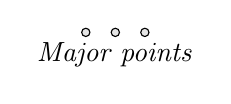
\begin{tikzpicture}[scale=.75]
\tkzDefPoints{1/0/A,1.5/0/B,2/0/C} 
\MajorPoints{A,B,C}
\node[anchor=north] at (1.5,0) {\textit{Major points}};
\end{tikzpicture}
%
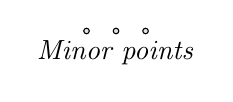
\begin{tikzpicture}[scale=.75]
\tkzDefPoints{1/0/A,1.5/0/B,2/0/C} 
\MinorPoints{A,B,C}
\node[anchor=north] at (1.5,0) {\textit{Minor points}};
\end{tikzpicture}

\subsection{Angle markers}

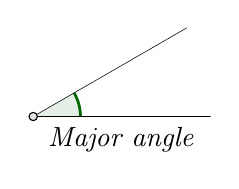
\begin{tikzpicture}[scale=.75]
\tkzDefPoints{0/0/O,3/0/x} \tkzDefPoint(30:3){y}
\MajorAngle{x,O,y} \MajorSegments{O,x O,y} \MajorPoints{O}
\node[anchor=north] at (1.5,0) {\textit{Major angle}};
\end{tikzpicture}
%
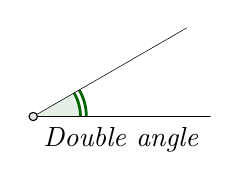
\begin{tikzpicture}[scale=.75]
\tkzDefPoints{0/0/O,3/0/x} \tkzDefPoint(30:3){y}
\DoubleAngle{x,O,y} \MajorSegments{O,x O,y} \MajorPoints{O}
\node[anchor=north] at (1.5,0) {\textit{Double angle}};
\end{tikzpicture}
%
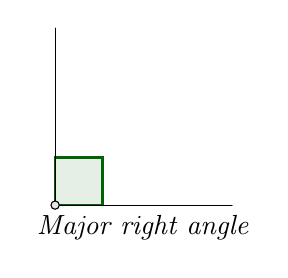
\begin{tikzpicture}[scale=.75]
\tkzDefPoints{0/0/O,3/0/x} \tkzDefPoint(90:3){y}
\MajorRightAngle{x,O,y} \MajorSegments{O,x O,y} \MajorPoints{O}
\node[anchor=north] at (1.5,0) {\textit{Major right angle}};
\end{tikzpicture}
%
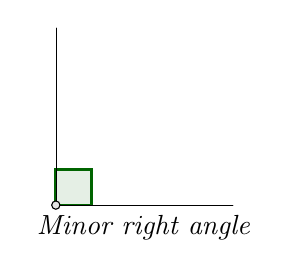
\begin{tikzpicture}[scale=.75]
\tkzDefPoints{0/0/O,3/0/x} \tkzDefPoint(90:3){y}
\MinorRightAngle{x,O,y} \MajorSegments{O,x O,y} \MajorPoints{O}
\node[anchor=north] at (1.5,0) {\textit{Minor right angle}};
\end{tikzpicture}
%
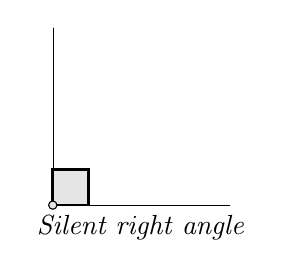
\begin{tikzpicture}[scale=.75]
\tkzDefPoints{0/0/O,3/0/x} \tkzDefPoint(90:3){y}
\SilentRightAngle{x,O,y} \MajorSegments{O,x O,y} \MajorPoints{O}
\node[anchor=north] at (1.5,0) {\textit{Silent right angle}};
\end{tikzpicture}


\subsection{Angle equality markers}

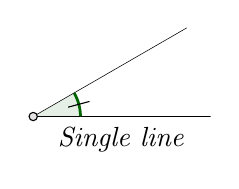
\begin{tikzpicture}[scale=.75]
\tkzDefPoints{0/0/O,3/0/x} \tkzDefPoint(30:3){y}
\MajorAngle{x,O,y} \MajorSegments{O,x O,y} \MajorPoints{O}
\tkzMarkAngles[color=AngleClr,size=.8,mark=|](x,O,y)
\node[anchor=north] at (1.5,0) {\textit{Single line}};
\end{tikzpicture}
%
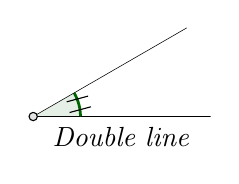
\begin{tikzpicture}[scale=.75]
\tkzDefPoints{0/0/O,3/0/x} \tkzDefPoint(30:3){y}
\MajorAngle{x,O,y} \MajorSegments{O,x O,y} \MajorPoints{O}
\tkzMarkAngles[color=AngleClr,size=.8,mark=||](x,O,y)
\node[anchor=north] at (1.5,0) {\textit{Double line}};
\end{tikzpicture}
%
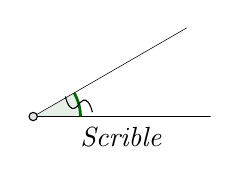
\begin{tikzpicture}[scale=.75]
\tkzDefPoints{0/0/O,3/0/x} \tkzDefPoint(30:3){y}
\MajorAngle{x,O,y} \MajorSegments{O,x O,y} \MajorPoints{O}
\tkzMarkAngles[color=AngleClr,size=.8,mark=s](x,O,y)
\node[anchor=north] at (1.5,0) {\textit{Scrible}};
\end{tikzpicture}
%
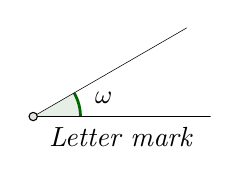
\begin{tikzpicture}[scale=.75]
\tkzDefPoints{0/0/O,3/0/x} \tkzDefPoint(30:3){y}
\MajorAngle{x,O,y} \MajorSegments{O,x O,y} \MajorPoints{O}
\tkzLabelAngles[scale=0.95,pos=1.3](x,O,y){$\omega$}
\node[anchor=north] at (1.5,0) {\textit{Letter mark}};
\end{tikzpicture}
%
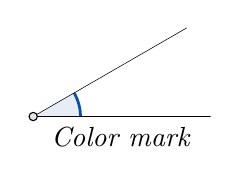
\begin{tikzpicture}[scale=.75]
\tkzDefPoints{0/0/O,3/0/x} \tkzDefPoint(30:3){y}
\MajorAngle[BlueClr]{x,O,y} \MajorSegments{O,x O,y} \MajorPoints{O}
\node[anchor=north] at (1.5,0) {\textit{Color mark}};
\end{tikzpicture}


Angle should be drawn below shape/line.

\subsection{Types of segments}
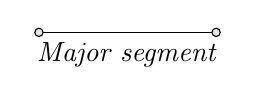
\begin{tikzpicture}[scale=.75]
\tkzDefPoints{0/0/A,3/0/B} 
\MajorSegments{A,B} \MajorPoints{A,B}
\node[anchor=north] at (1.5,0) {\textit{Major segment}};
\end{tikzpicture}
%
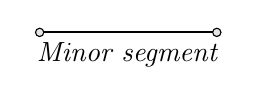
\begin{tikzpicture}[scale=.75]
\tkzDefPoints{0/0/A,3/0/B} 
\MinorSegments{A,B} \MajorPoints{A,B}
\node[anchor=north] at (1.5,0) {\textit{Minor segment}};
\end{tikzpicture}
%
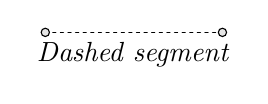
\begin{tikzpicture}[scale=.75]
\tkzDefPoints{0/0/A,3/0/B} 
\DashedSegments{A,B} \MajorPoints{A,B}
\node[anchor=north] at (1.5,0) {\textit{Dashed segment}};
\end{tikzpicture}
%
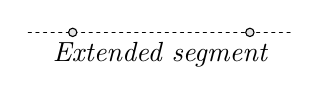
\begin{tikzpicture}[scale=.75]
\tkzDefPoints{0/0/A,3/0/B} 
\tkzDrawSegment[line width=0.55pt,color=black,dashed,dash pattern=on 1pt off 1.75pt,add=0.25 and 0.25](A,B) \MajorPoints{A,B}
\node[anchor=north] at (1.5,0) {\textit{Extended segment}};
\end{tikzpicture}

\subsection{Types of segment equality}
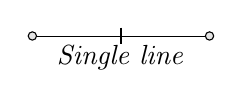
\begin{tikzpicture}[scale=.75]
\tkzDefPoints{0/0/A,3/0/B} 
\MajorSegments{A,B} \MajorPoints{A,B}
\tkzMarkSegments[mark=|,size=3](A,B)
\node[anchor=north] at (1.5,0) {\textit{Single line}};
\end{tikzpicture}
%
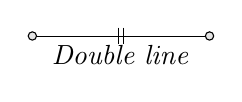
\begin{tikzpicture}[scale=.75]
\tkzDefPoints{0/0/A,3/0/B} 
\MajorSegments{A,B} \MajorPoints{A,B} \tkzMarkSegments[mark=||,size=3](A,B)
\node[anchor=north] at (1.5,0) {\textit{Double line}};
\end{tikzpicture}
%
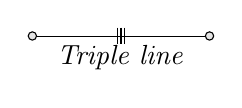
\begin{tikzpicture}[scale=.75]
\tkzDefPoints{0/0/A,3/0/B} 
\MajorSegments{A,B} \MajorPoints{A,B} \tkzMarkSegments[mark=|||,size=3](A,B)
\node[anchor=north] at (1.5,0) {\textit{Triple line}};
\end{tikzpicture}
%
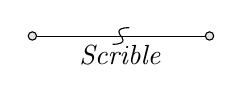
\begin{tikzpicture}[scale=.75]
\tkzDefPoints{0/0/A,3/0/B} 
\MajorSegments{A,B} \MajorPoints{A,B} \tkzMarkSegments[mark=s,size=3](A,B)
\node[anchor=north] at (1.5,0) {\textit{Scrible}};
\end{tikzpicture}
%
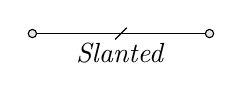
\begin{tikzpicture}[scale=.75]
\tkzDefPoints{0/0/A,3/0/B} 
\MajorSegments{A,B} \MajorPoints{A,B} \tkzMarkSegments[mark=s|,size=3](A,B)
\node[anchor=north] at (1.5,0) {\textit{Slanted}};
\end{tikzpicture}
%
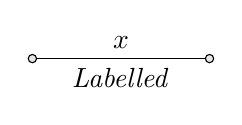
\begin{tikzpicture}[scale=.75]
\tkzDefPoints{0/0/A,3/0/B} 
\MajorSegments{A,B} \MajorPoints{A,B} \tkzLabelSegment[above](A,B){$x$}
\node[anchor=north] at (1.5,0) {\textit{Labelled}};
\end{tikzpicture}
%


\subsection{Types of circles}

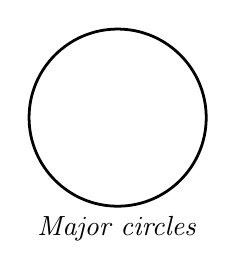
\begin{tikzpicture}[scale=.75]
\tkzDefPoints{1.5/1.5/O,1.5/0/A} 
\MajorCircles{O,A}
\node[anchor=north] at (1.5,0) {\textit{Major circles}};
\end{tikzpicture}
%
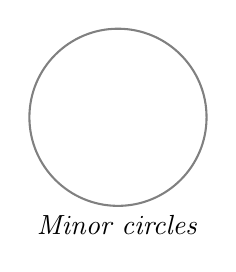
\begin{tikzpicture}[scale=.75]
\tkzDefPoints{1.5/1.5/O,1.5/0/A} 
\MinorCircles{O,A}
\node[anchor=north] at (1.5,0) {\textit{Minor circles}};
\end{tikzpicture}
%
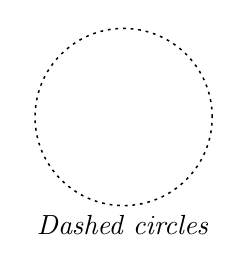
\begin{tikzpicture}[scale=.75]
\tkzDefPoints{1.5/1.5/O,1.5/0/A} 
\DashedCircles{O,A}
\node[anchor=north] at (1.5,0) {\textit{Dashed circles}};
\end{tikzpicture}
%
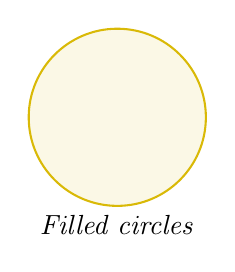
\begin{tikzpicture}[scale=.75]
\tkzDefPoints{1.5/1.5/O,1.5/0/A} 
\FilledCircles[YellowClr]{O,A}
\node[anchor=north] at (1.5,0) {\textit{Filled circles}};
\end{tikzpicture}
%

\subsection{Types of polygons}

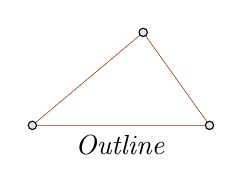
\begin{tikzpicture}[scale=.75]
\tkzDefPoints{0/0/A,3/0/B} \tkzDefPoint(40:2.45){C}

\tkzDrawPolygon[color=ShapeClr](A,B,C)
\MajorPoints{A,B,C}
\node[anchor=north] at (1.5,0) {\textit{Outline}};
\end{tikzpicture}
%
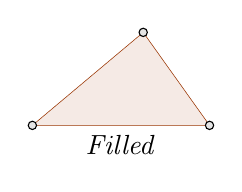
\begin{tikzpicture}[scale=.75]
\tkzDefPoints{0/0/A,3/0/B} \tkzDefPoint(40:2.45){C}

\tkzFillPolygon[fill=ShapeClr,fill opacity=0.1](C,A,B)
\tkzDrawPolygon[color=ShapeClr](A,B,C)
\MajorPoints{A,B,C}

\node[anchor=north] at (1.5,0) {\textit{Filled}};
\end{tikzpicture}
%

\begin{tikzpicture}[scale=.75]
\tkzDefPoint(140:1){P1}
\tkzDefPoint(102:1){P2}
\tkzDefPoint(45:1){P3}
\tkzDefPoint(-20:1){P4}
\tkzDefPoint(-40:1){P5}
\tkzDefPoint(-110:1){Pnn}
\tkzDefPoint(-175:1){Pn}


\tkzFillPolygon[fill=ShapeClr,fill opacity=0.1](P1,P2,P3,P4,P5,Pnn,Pn)

\tkzDrawSegments[line width=1pt,color=ShapeClr](Pnn,Pn Pn,P1 P1,P2 P2,P3 P3,P4 P4,P5)

\tkzLabelSegment[sloped](Pnn,P5){$\ldots$}
\node[anchor=north] at (0,-1.2) {\textit{General}};
\end{tikzpicture}

\subsection{Types of labels}


\begin{tikzpicture}[scale=.75]
\tkzDefPoints{1.5/0/A}
\tkzLabelPoint[above](A){$\rm A$}
\node[anchor=north] at (1.5,0) {\textit{Major point}};
\end{tikzpicture}
%
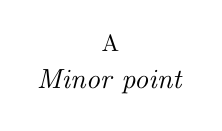
\begin{tikzpicture}[scale=.75]
\tkzDefPoints{1.5/0/A}
\tkzLabelPoint[scale=0.85,above](A){$\rm A$}
\node[anchor=north] at (1.5,0) {\textit{Minor point}};
\end{tikzpicture}
%
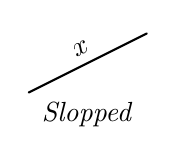
\begin{tikzpicture}[scale=.75]
\tkzDefPoints{0.5/0/A,2.5/1/B}
\MinorSegments{A,B}
\tkzLabelSegment[sloped,above](A,B){$x$}
\node[anchor=north] at (1.5,0) {\textit{Slopped}};
\end{tikzpicture}
%

\subsection{Standard colors}

\newcommand{\ColorBox}[2]{%
\begin{tikzpicture}[scale=.75]
\tkzDefPoints{0.5/0/A,2.5/0/B,2.5/1/C,0.5/1/D}
\tkzFillPolygon[fill=#1,fill opacity=0.1](A,B,C,D)
\tkzDrawPolygon[color=#1,line width=0.2](A,B,C,D)
\node[anchor=north] at (1.5,0) {\textit{#2}};
\end{tikzpicture}}

\ColorBox{ShapeClr}{Orange}\quad%
\ColorBox{GreenClr}{Green}\quad%
\ColorBox{BlueClr}{Blue}\quad%
\ColorBox{YellowClr}{Yellow}\quad%
\ColorBox{RedClr}{Red}\quad%
\ColorBox{black}{Black}%

\section{Common mistakes}

It would be nice to have a set of (soft) rules/guidelines on when to use certain types of components.

\newtcolorbox{donts}[2][]{capture=hbox,colbacktitle=red!75!white,colframe=red!70!black,colback=red!5!white,
title={\xmark #2},every float=\centering,#1}

\newtcolorbox{dos}[2][]{capture=hbox,colbacktitle=green!90!black,colframe=green!65!black,colback=green!5!white,
title={\cmark #2},every float=\centering,#1}

\begin{donts}[label={fig:Qp}]{Angles after segments}
 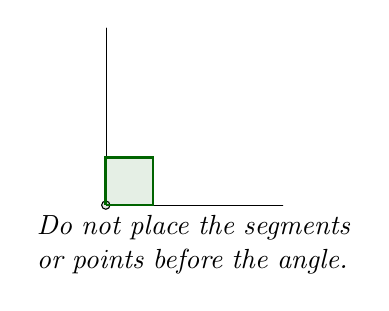
\begin{tikzpicture}[scale=.75]
\tkzDefPoints{0/0/O,3/0/x} \tkzDefPoint(90:3){y}
\MajorSegments{O,x O,y} \MajorPoints{O} \MajorRightAngle{x,O,y}
\node[anchor=north,text width=4cm] at (1.5,0) {\textit{Do not place the segments or points before the angle.}};
\end{tikzpicture}

 \end{donts}%
 \begin{dos}[label={fig:Qp}]{Mark cyclic quads}
 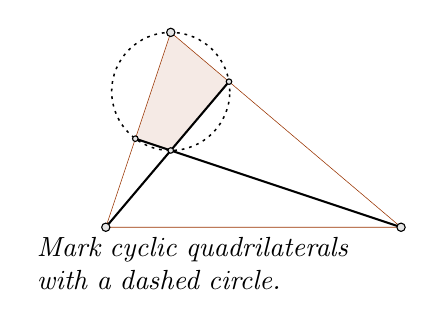
\begin{tikzpicture}[scale=.75]
\tkzDefPoints{0/0/B,1.1/3.3/A,5/0/C}
\tkzDrawPolygon[color=ShapeClr](A,B,C)
\tkzDefTriangleCenter[ortho](A,B,C)\tkzGetPoint{H}
\tkzDefPointBy[projection=onto A--C](H)\tkzGetPoint{HB}
\tkzDefPointBy[projection=onto A--B](H)\tkzGetPoint{HC}
\tkzDefTriangleCenter[circum](HB,HC,H)\tkzGetPoint{O}
\tkzFillPolygon[fill=ShapeClr,fill opacity=0.1](A,HB,H,HC)
\MinorSegments{B,HB C,HC}
\DashedCircles{O,H}
\MajorPoints{A,B,C}
\MinorPoints{HB,HC,H}
\node[anchor=north,text width=4cm] at (1.5,0) {\textit{Mark cyclic quadrilaterals with a dashed circle.}};
\end{tikzpicture}
\end{dos}

\begin{dos}{Line of a segment}
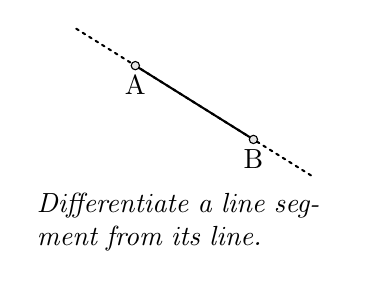
\begin{tikzpicture}[scale=.75]
\tkzDefPoints{0/0/A,2/-1.25/B} % The endpoints of the line segment.

\tkzDrawSegments[line width=0.75pt,color=black](A,B)
\tkzDrawSegment[line width=0.75pt,color=black,dashed,dash pattern=on 1pt off 1.75pt,add = 0.5 and 0.5](A,B)

\tkzDrawPoints[size=3](A,B)

\tkzLabelPoint[below](A){$\rm A$}
\tkzLabelPoint[below](B){$\rm B$}

\node[anchor=north,text width=4cm] at (1,-2) {\textit{Differentiate a line segment from its line.}};
\end{tikzpicture}
\end{dos}

\begin{dos}{Extend a line}
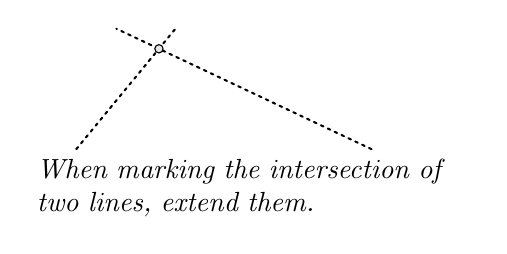
\begin{tikzpicture}[scale=.75]
\tkzDefPoints{0/0/B,1.4/1.7/A,5/0/C}

\tkzDrawSegments[line width=0.75pt,color=black,dashed,dash pattern=on 1pt off 1.75pt,add = 0 and 0.2](B,A C,A)

\MajorPoints{A}
\node[anchor=north,text width=5.5cm] at (3,0) {\textit{When marking the intersection of two lines, extend them.}};
\end{tikzpicture}
\end{dos}


\section{Some ideas/questions}

\begin{itemize}
 \item Should we always mark an angle referred during a proof?
 \item Should all equal angles be highlighted?
 \item When should we add a label to an angle?
 \item When to fill a shape?
 \item When to use a color to mark an angle?
 \item How many angle equality markers are too may for a single figure?
 \item When is it appropriate to use a second figure for the same proof?
\end{itemize}


\end{document}
